% !TeX root = ../thesis.tex

\chapter{Evaluation}
\label{sec:evaluation}
Im Vorausgegangenen wurde der Aufbau des Senders umfangreich geschildert. Nun soll dieser in seiner Funktionalität evaluiert werden. Zunächst sollten hierfür die Eigenschaften der einzelnen Verstärkerstufen im analogen Signalverarbeitungsschaltkreis erprobt und die Simulationen verifiziert werden. Als Testsignal wurde mithilfe eines Frequenzgenerators ein Sinussignal generiert, welches sich auf Grund seiner bekannten Form sehr gut zur Überprüfung eignet. Das Sinussignal wurde mit einer Frequenz von 15kHz generiert, da dies etwa im Bereich der Frequenz des später gesendeten Nutzsignals liegt. 


\begin{figure}[h]
	\centering
	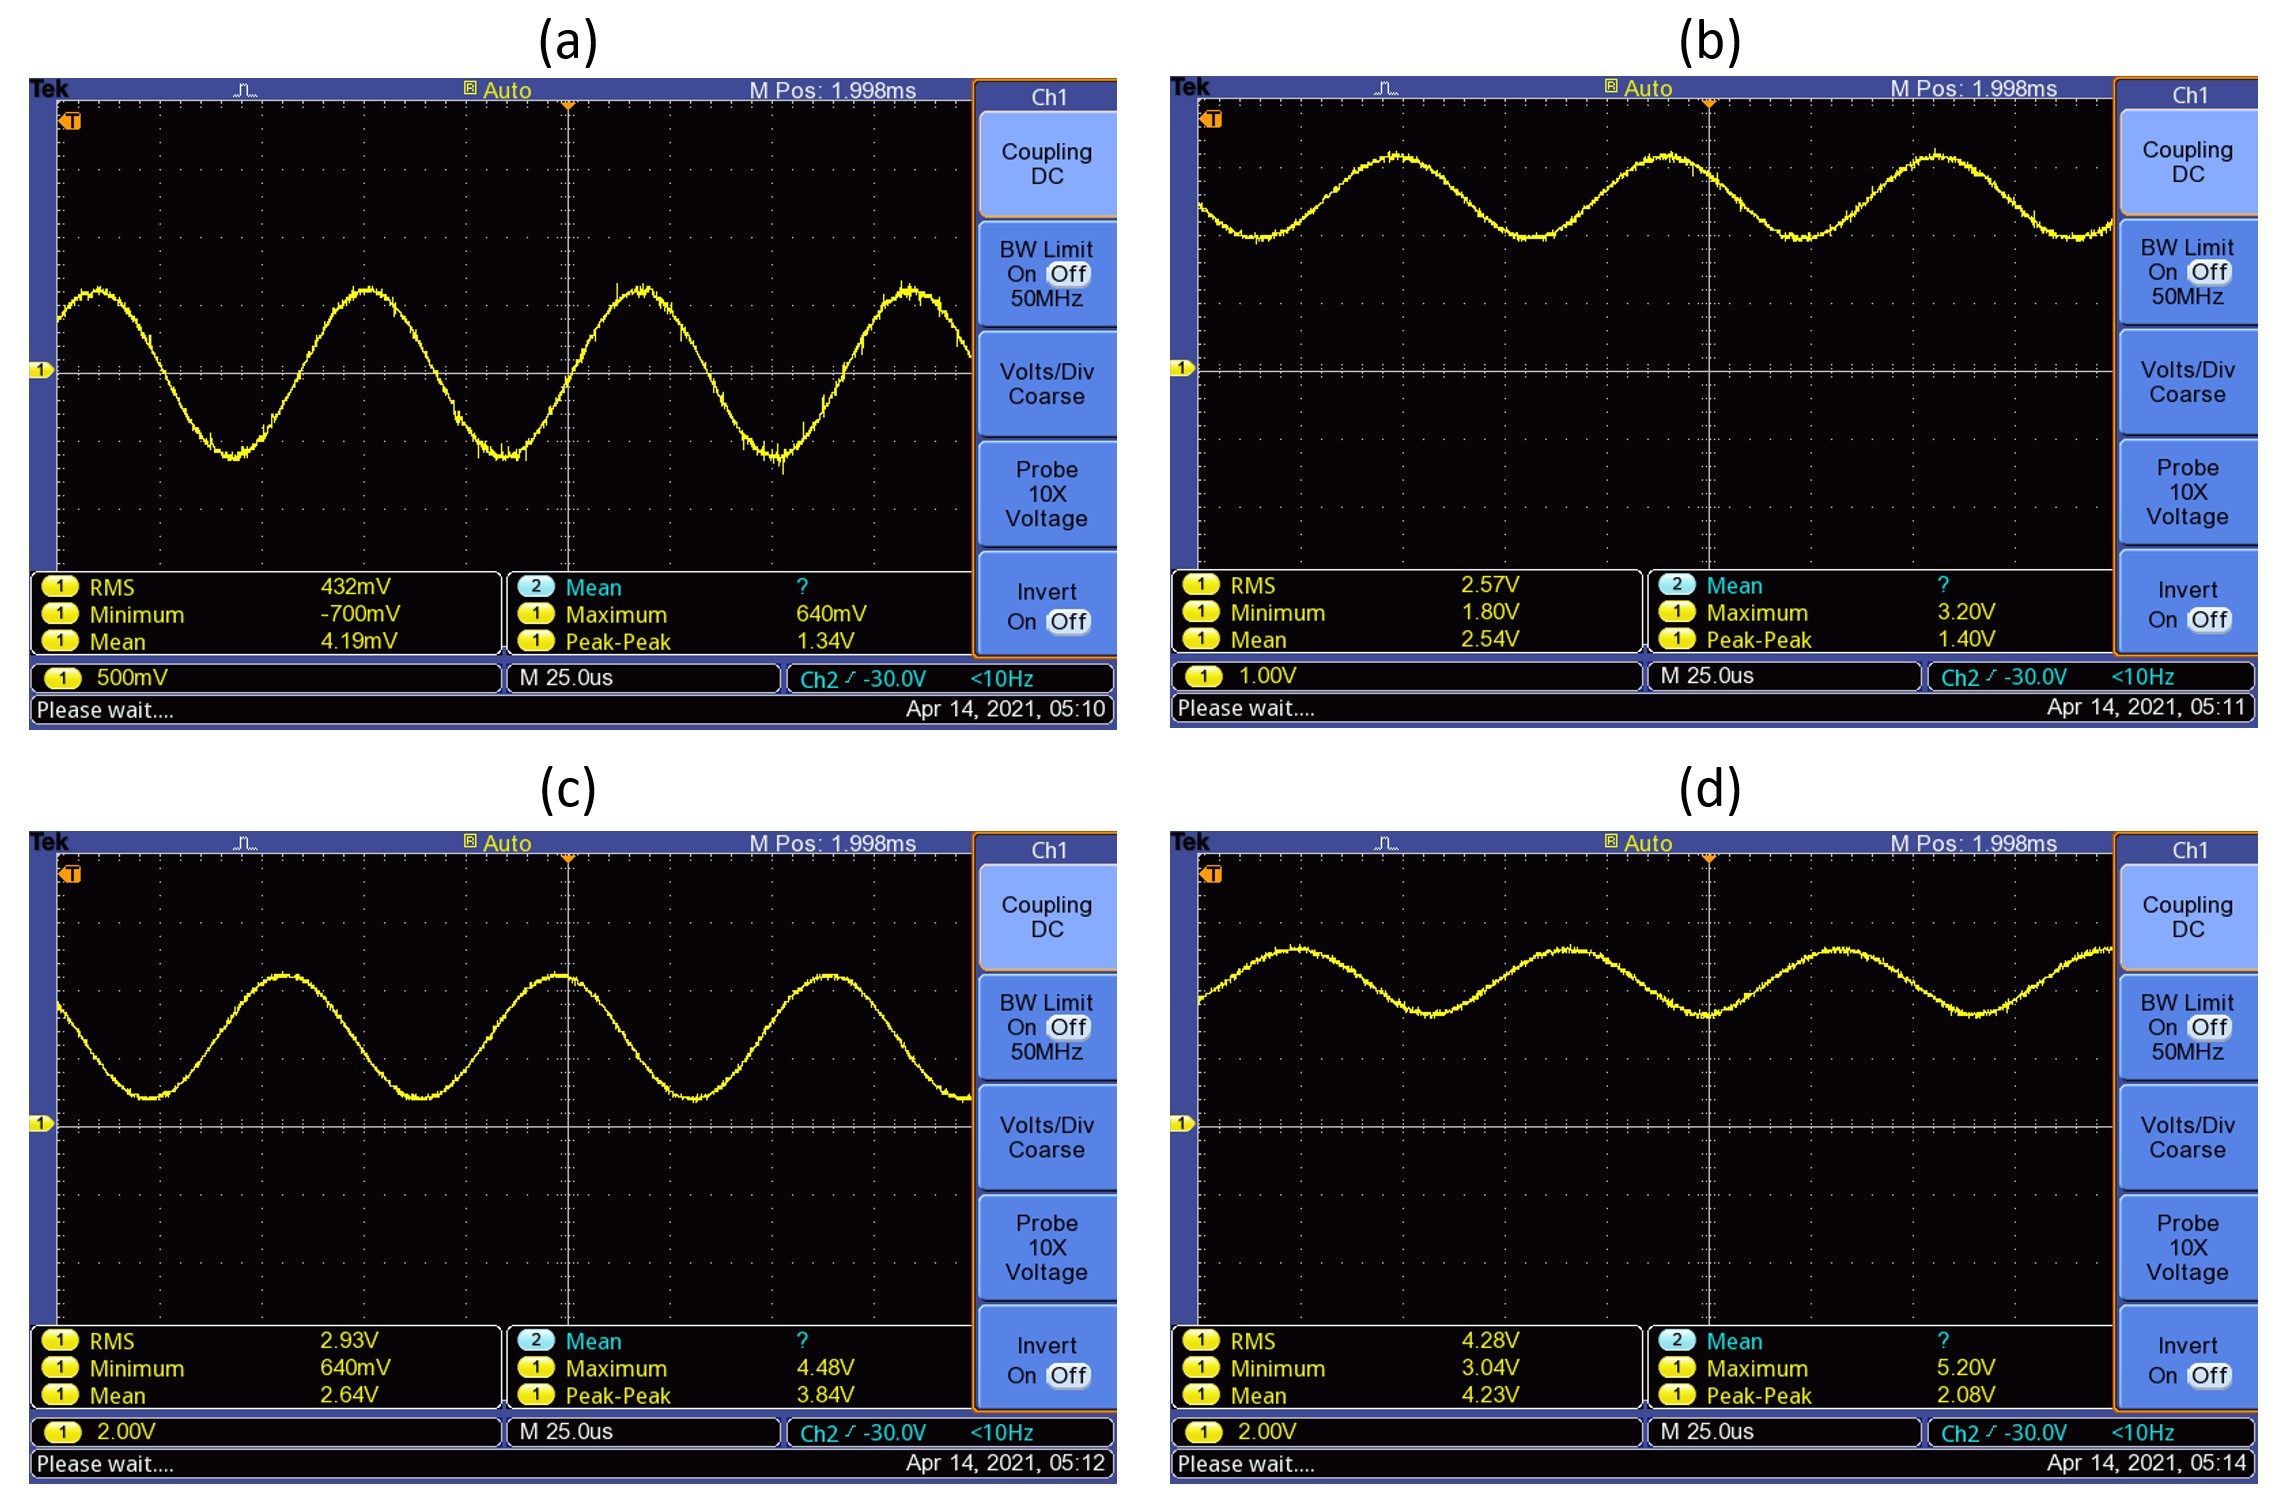
\includegraphics[width = 1 \textwidth]{stufenfkt.jpg}
	\caption[Veranschaulichung der Ausgabe der Stufen mit dem Testsignal]{Veranschaulichung der Ausgabe der Stufen mit dem Testsignal}
	\label{fig:stufeneva}
\end{figure}

(a) aus Abbildung~\ref{fig:stufeneva} veranschaulicht das Eingangssignal der Schaltung. Dabei handelt es sich um das reine Sinussignal, welches aus der Soundkarte des Computers moduliert wird. Im Teil (b) der genannten Abbildung wird dieses Eingangssignal wie erwartet nach dem \gls{acr:DC}-Abblockkondensator mit einem fest eingestellten Offset versehen. Teil (c) der Abbildung zeigt das verstärkte Eingangsignal am Ausgang der ersten Verstärkerstufe. Dabei wurde die \gls{acr:LED} nahe dem Arbeitspunkt betrieben, was dafür sorgt dass die Amplitude, innerhalb der gegebenen Spannungsgrenzen, beinahe maximal verstärkt wird. Im letzten Abschnitt der Abbildung ~\ref{fig:stufeneva} wird das Sinussignal um den vom Potentiometer eingestellten Offset auf eine Spannungswert von 4,23V verschoben. Die Abbildungen bestätigen die vorher simulierten und approximierten Effekte der analogen Signalverarbeitungsschaltung auf das Testsignal. 


Nach erfolgreichem Testen der verschiedenen Verstärkerstufen, war es das Ziel, der Schaltung das \gls{acr:DRM}- Nutzsignal zuzuführen und dieses Anhand verschiedener Faktoren zu analysieren. Zunächst wurde hierbei jedoch noch die Funktionalität der Amplitudenregelung untersucht. Hierfür wurden vier verschiedene Helligkeitsstufen über den Offset eingestellt und nachgemessen.

\begin{figure}[h]
	\centering
	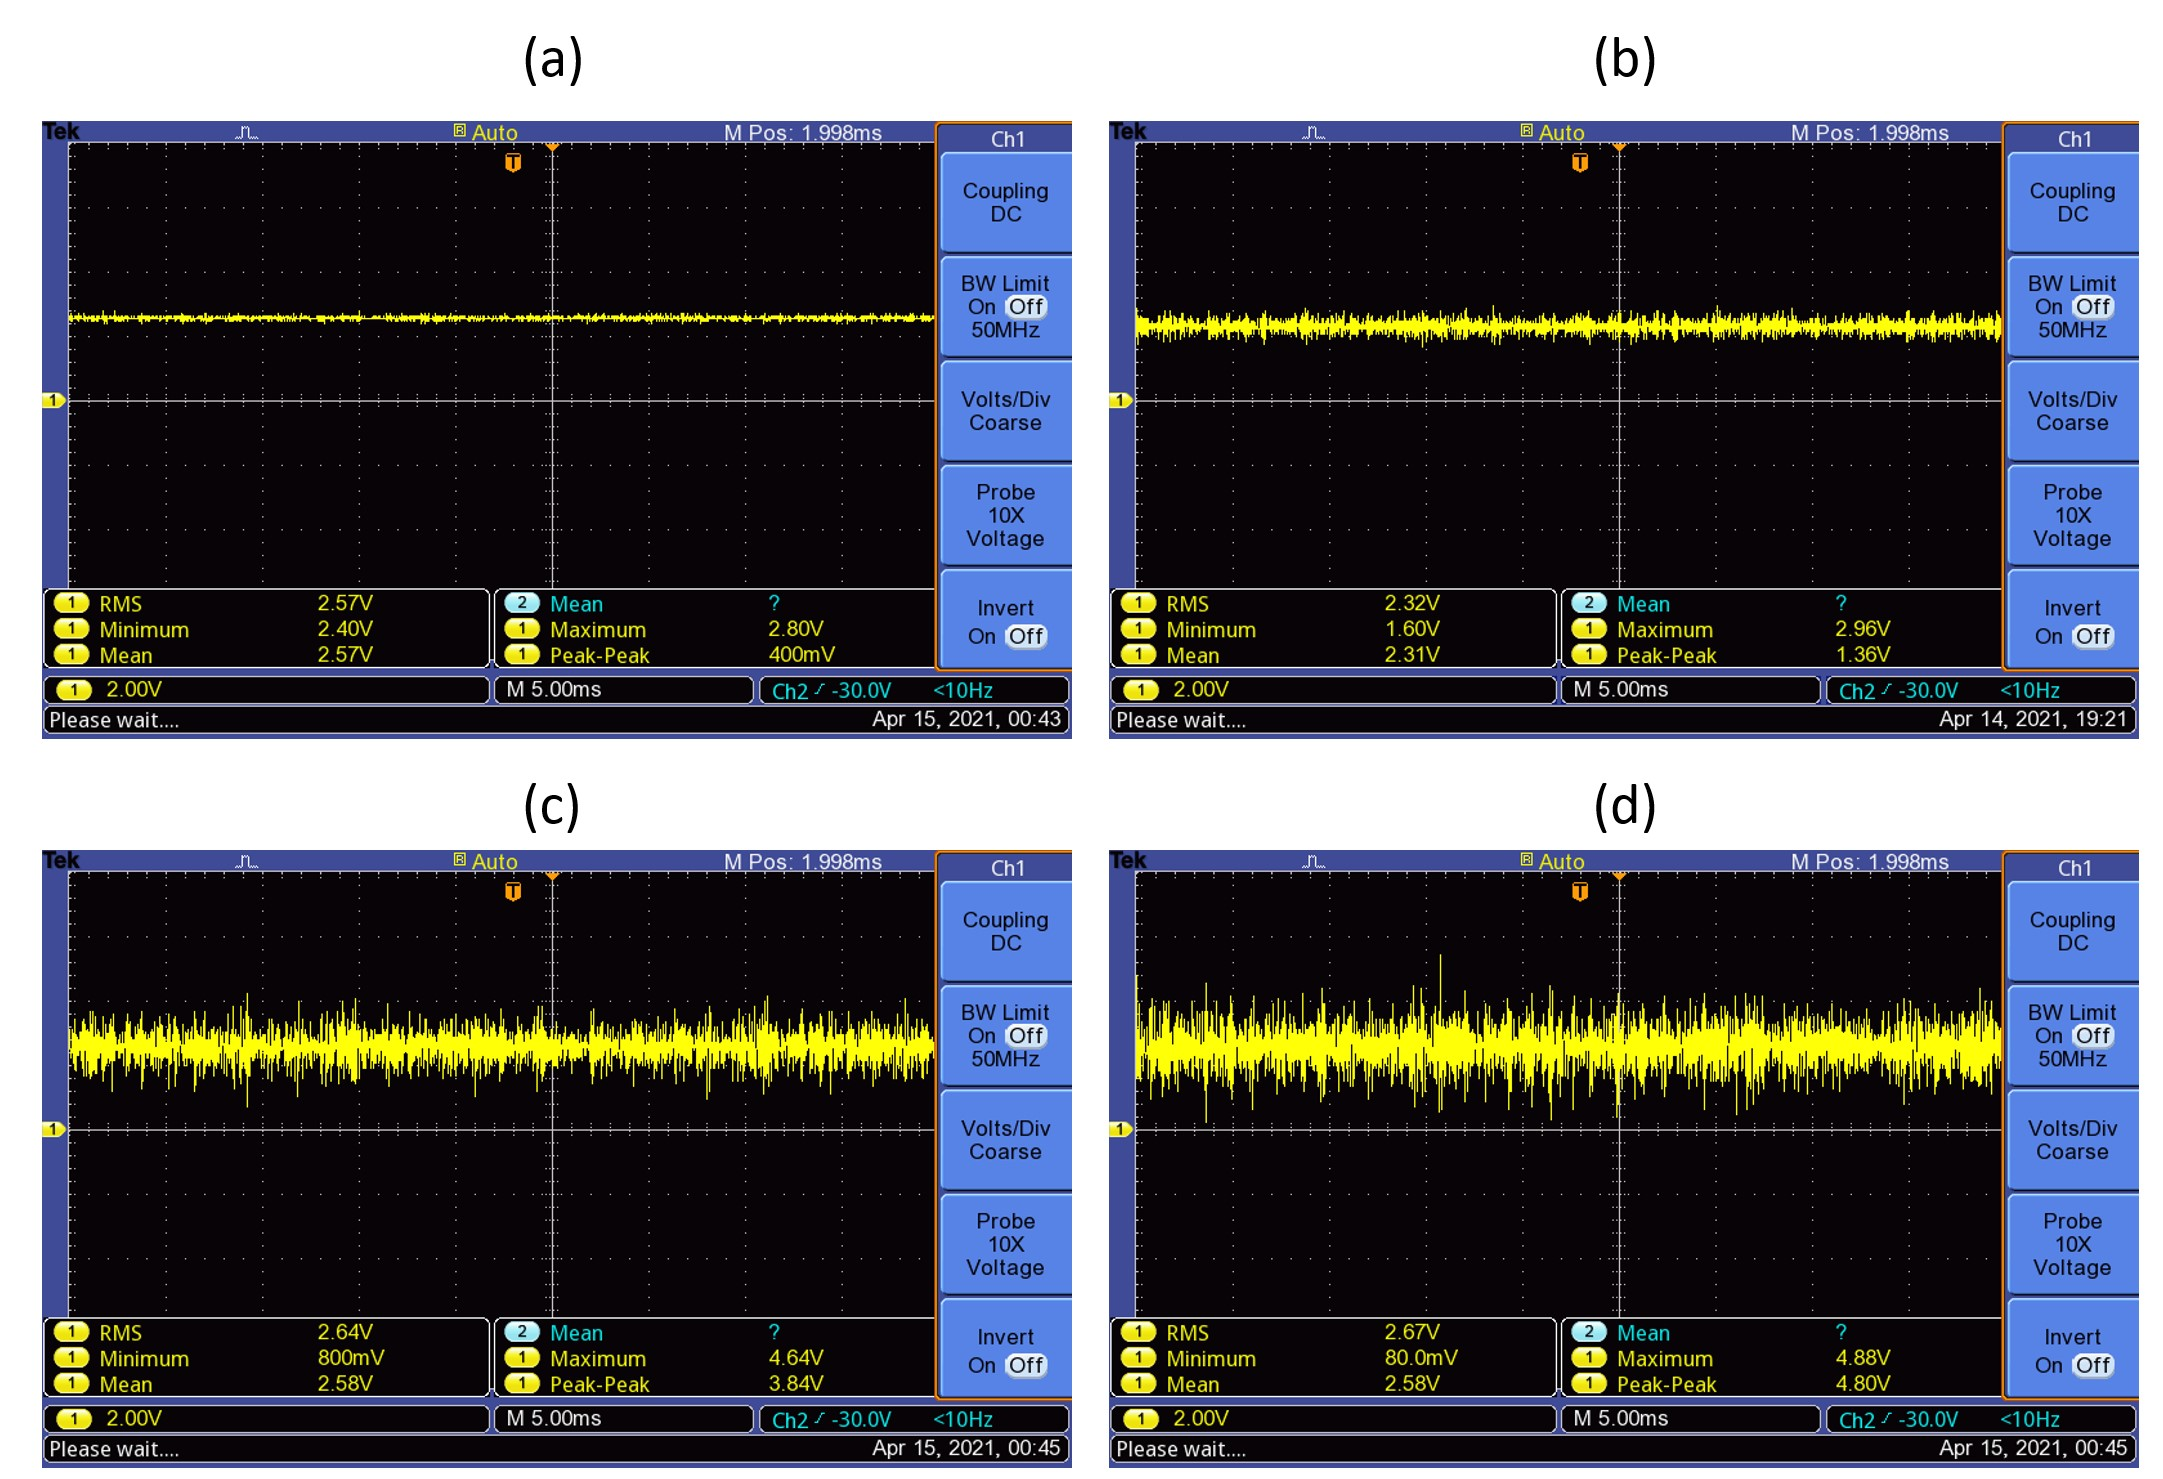
\includegraphics[width = 1 \textwidth]{signaleva.jpg}
	\caption[Amplitudenregelung in vier Schritten]{Amplitudenregelung in vier Schritten}
	\gls{online:Eigen}
	\label{fig:Amplitudenregelung}
\end{figure}

Beim erhöhen des Offsets ausgehend vom Nullpunkt in Richtung des Arbeitspunktes konnte bestimmt werden, dass mit steigendem Offset auch die Amplitudenverstärkung zunimmt. Damit konnte das Ziel der Amplitudenregelung auch erreicht werden. womit sich die Funktion des S da dort Amplitude einen größeren Aktionsradius besitzt. In Folge dessen, konnte die Auswirkung der Amplitude auf das Spektrum des \gls{acr:DRM}-Nutzsignals veranschaulicht werden. Dieser Schritt wird in Abbildung~\ref{fig:speki} dargestellt. Mit steigender Amplitude hebt sich das Signal im Spektrum immer weiter hervor und wird somit an seinen charakterisierenden Stellen ausgeprägter erkennbar. Hierbei ist die im Dream Transmitter eingestellte Trägerfrequenz von 12kHz und die Bandbreite von 10kHz deutlich zu sehen.


\begin{figure}[h]
	\centering
	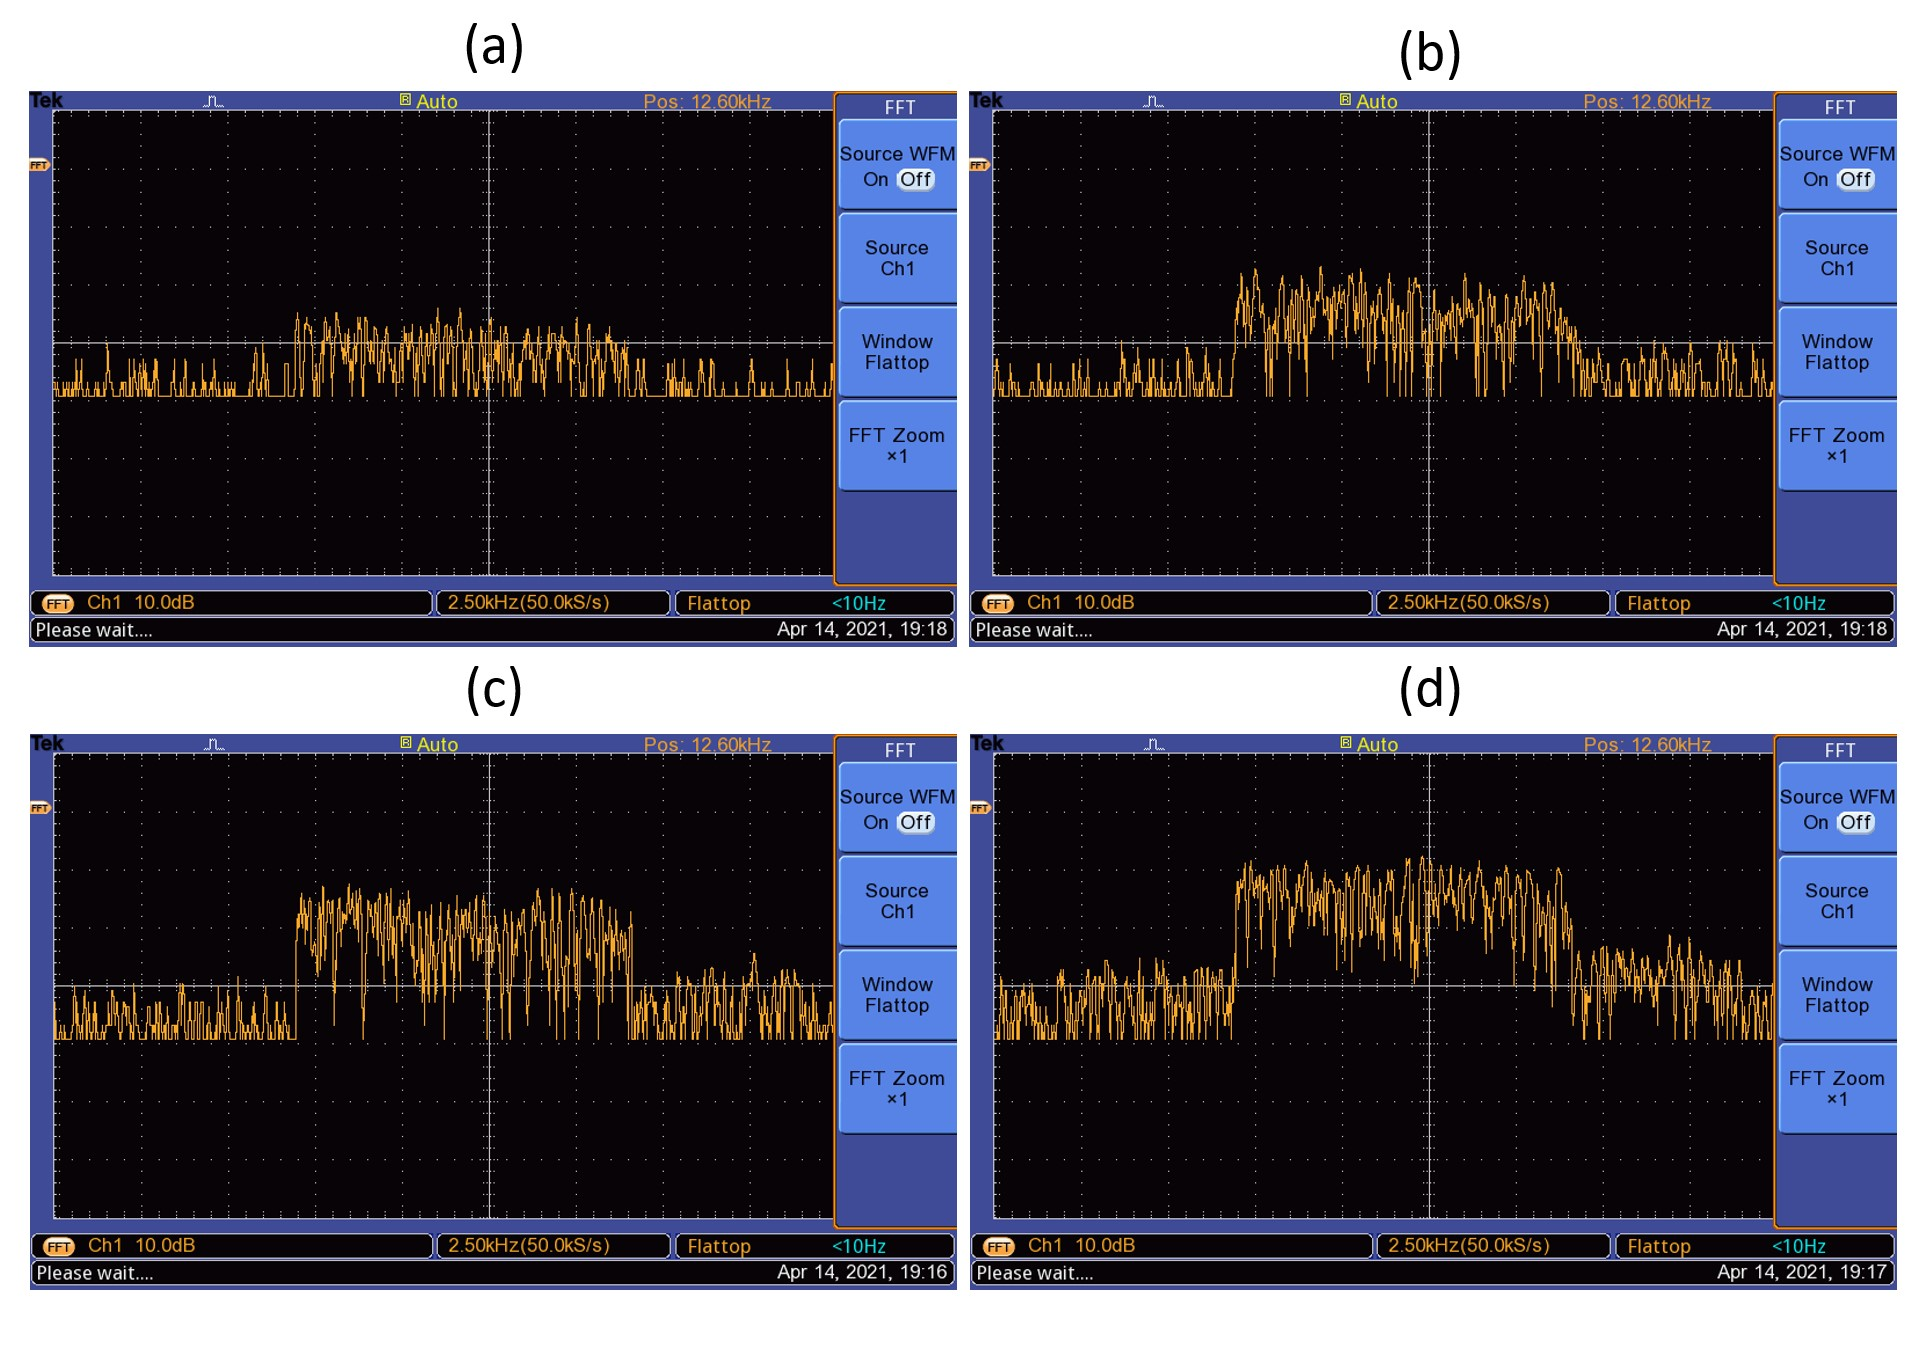
\includegraphics[width = 1 \textwidth]{spekeva.jpg}
	\caption[Amplitudenregelung in vier Schritten - Spektrum]{Amplitudenregelung in vier Schritten - Spektrum}\gls{online:Eigen}
	\label{fig:speki}
\end{figure}


Im Anschluss dienen die in Abbildung~\ref{fig:dreamtxeinstellung} illustrierten und in Tabelle~\ref{tab:dreamparam} näher erläuterten vom Sender einstellbaren Parameter zur Evaluierung des Signals auf der Empfängerseite. Diese wurden unter verschiedenen Kriterien evaluiert. Hierzu diente beispielsweise das Erreichen eines höheren Datendurchsatzes. Diese Messungen wurden unter optimalen Bedingungen durchgeführt. So wurden fremde Lichtquellen, wie die Deckenbeleuchtung und auch das Tageslicht, bewusst minimiert. Zur Übertragung wurde in dieser Evaluation grundsätzlich eine Zwischenfrequenz von 12 kHz sowie eine Bandbreite des Signals von 10 kHz verwendet.

Durch das Testen der verschiedenen Robustness Modes konnte die Wahl auf Mode B beschränkt werden, da hier experimentell die besten Übertragungsresultate erzielt werden konnten. Mode A, bei welchem ein höhere Datenrate von 34,8 kbps übertragen werden kann, hat sich in den Übertragungstests als weniger störresistent herausgestellt. Modes C und D hingegen, sind Störungen gegenüber weniger anfällig. Dies jedoch zu einer geringen Datenrate, worunter die Audioqualität der Übertragung teilweise stark leidet. Mode B liefert hier als Folge dessen den besten Kompromiss zwischen Audioqualität und Störresistenz.

Als variable Parameter dienen nun also die Modulationsart der \gls{acr:MSC}s, sowie die Protection und Interleaver Modes. Tabelle~\ref{tab:drmevaluationmax} veranschaulicht die Messergebnisse der verschiedenen Konstellationen der Einstellungen des Senders. Hierbei konnte ermittelt werden, dass bei einer Erhöhung des Protection Levels wie erwartet die Datenrate der Übertragung sinkt. Dies ist auf die in Unterkapitel~\ref{subsec:drm} erwähnte Coderate zurückzuführen. Je höher also das Protection Level (wobei 0 hier den größten Schutz bietet), desto geringer ist letztendlich die Code-Rate, also das Verhältnis der Informationssymbole zur Länge der Wörter. Es werden demnach bei einem höheren Schutz mehr Redundante Bits in die Daten miteinkodiert, um die eigentlich interessanten Nutzdaten bei der Dekodierung besser rekonstruieren zu können. 



\begin{table}[H]
	\begin{center}
		\begin{tabular}{cccc}
			\toprule
			\textbf{Datenrate [kbps]} & \textbf{Modulation}& \textbf{\gls{acr:MSC} Protection Level} & \textbf{\gls{acr:MSC} Interleaver Mode}\\
			\midrule
			11.64 & 16-\gls{acr:QAM} & 0 & 0.4s (Short Intervall)\\
			14.56 &16-\gls{acr:QAM} & 1 & 0.4s (Short Intervall)\\
			11.64 & 16-\gls{acr:QAM} & 0 & 2s (Long Intervall)\\
			14.56 & 16-\gls{acr:QAM} & 1 & 2s (Long Intervall) \\
			17.46 & 64-\gls{acr:QAM} & 0 & 0.4s (Short Intervall)\\
			20.96 & 64-\gls{acr:QAM} & 1 & 0.4s (Short Intervall)\\
			24.74 & 64-\gls{acr:QAM} & 2 & 0.4s (Short Intervall)\\
			27.44 & 64-\gls{acr:QAM} & 3 & 0.4s (Short Intervall) \\
			17.46 & 64-\gls{acr:QAM} & 0 & 2s (Long Intervall)\\
			20.96 & 64-\gls{acr:QAM} & 1 & 2s (Long Intervall)\\
			24.74 & 64-\gls{acr:QAM} & 2 & 2s (Long Intervall)\\
			27.44 & 64-\gls{acr:QAM} & 3 & 2s (Long Intervall) \\
			\bottomrule
		\end{tabular}
		\caption{Evaluation des Signals auf eine Übertragung über 5m}\gls{online:dream}
		\label{tab:drmevaluationmax}
	\end{center}
\end{table}





Zur Veranschaulichung und Bewertung der Übertragung eines \gls{acr:DRM}-Signals wurden im folgenden die Konstellationsdiagramme für \gls{acr:MSC} (16-\gls{acr:QAM}),\gls{acr:FAC} (16-\gls{acr:QAM}) und \gls{acr:SDC} (4-\gls{acr:QAM}) dargestellt. Teil (a) der Abbildungsreihe~\ref{fig:msc} -~\ref{fig:fac} beschreibt eine missglückte Darstellung bei welcher Konstellationspunkte nicht mehr fehlerfrei ihrer ursprünglichen Position zugeordnet werden können, wodurch eine fehlerfreie Übertragung nicht zu Stande kommen kann. (b) hingegen beschreibt den erfolgreichen Übertragungsfall, da hier Konstellationspunkte nur kleine Streuungen erfahren und noch relativ fehlerfrei zugeordnet werden können.

Wie in Teil (b) der Abbildungsreihe zu sehen ist, schwankt die Phase nur in einem Bereich, in dem die empfangenen Symbole noch sicher einem der vordefinierten Symbole zugeordnet werden können. Bei stärkerer Schwankung wie in Teil (a) veranschaulicht, ist diese Zuordnung nicht mehr möglich. Um einem Effekt der Phasenverschiebung entgegen zu wirken, werden bei solchen Übertragungen Präambeln benutzt. Dabei handelt es sich um vordefinierte Rahmen in Form einer festgelegten Bitfolge, die sowohl Sender als auch Empfänger entsprechend vorliegt. Hierdurch kann der Empfänger seine Parameter so anpassen, bis sie mit der Präambel einhergehen. So kann die richtige Phase detektiert und der Phasenversatz kompensiert werden.

\begin{figure}[H]
	\centering
	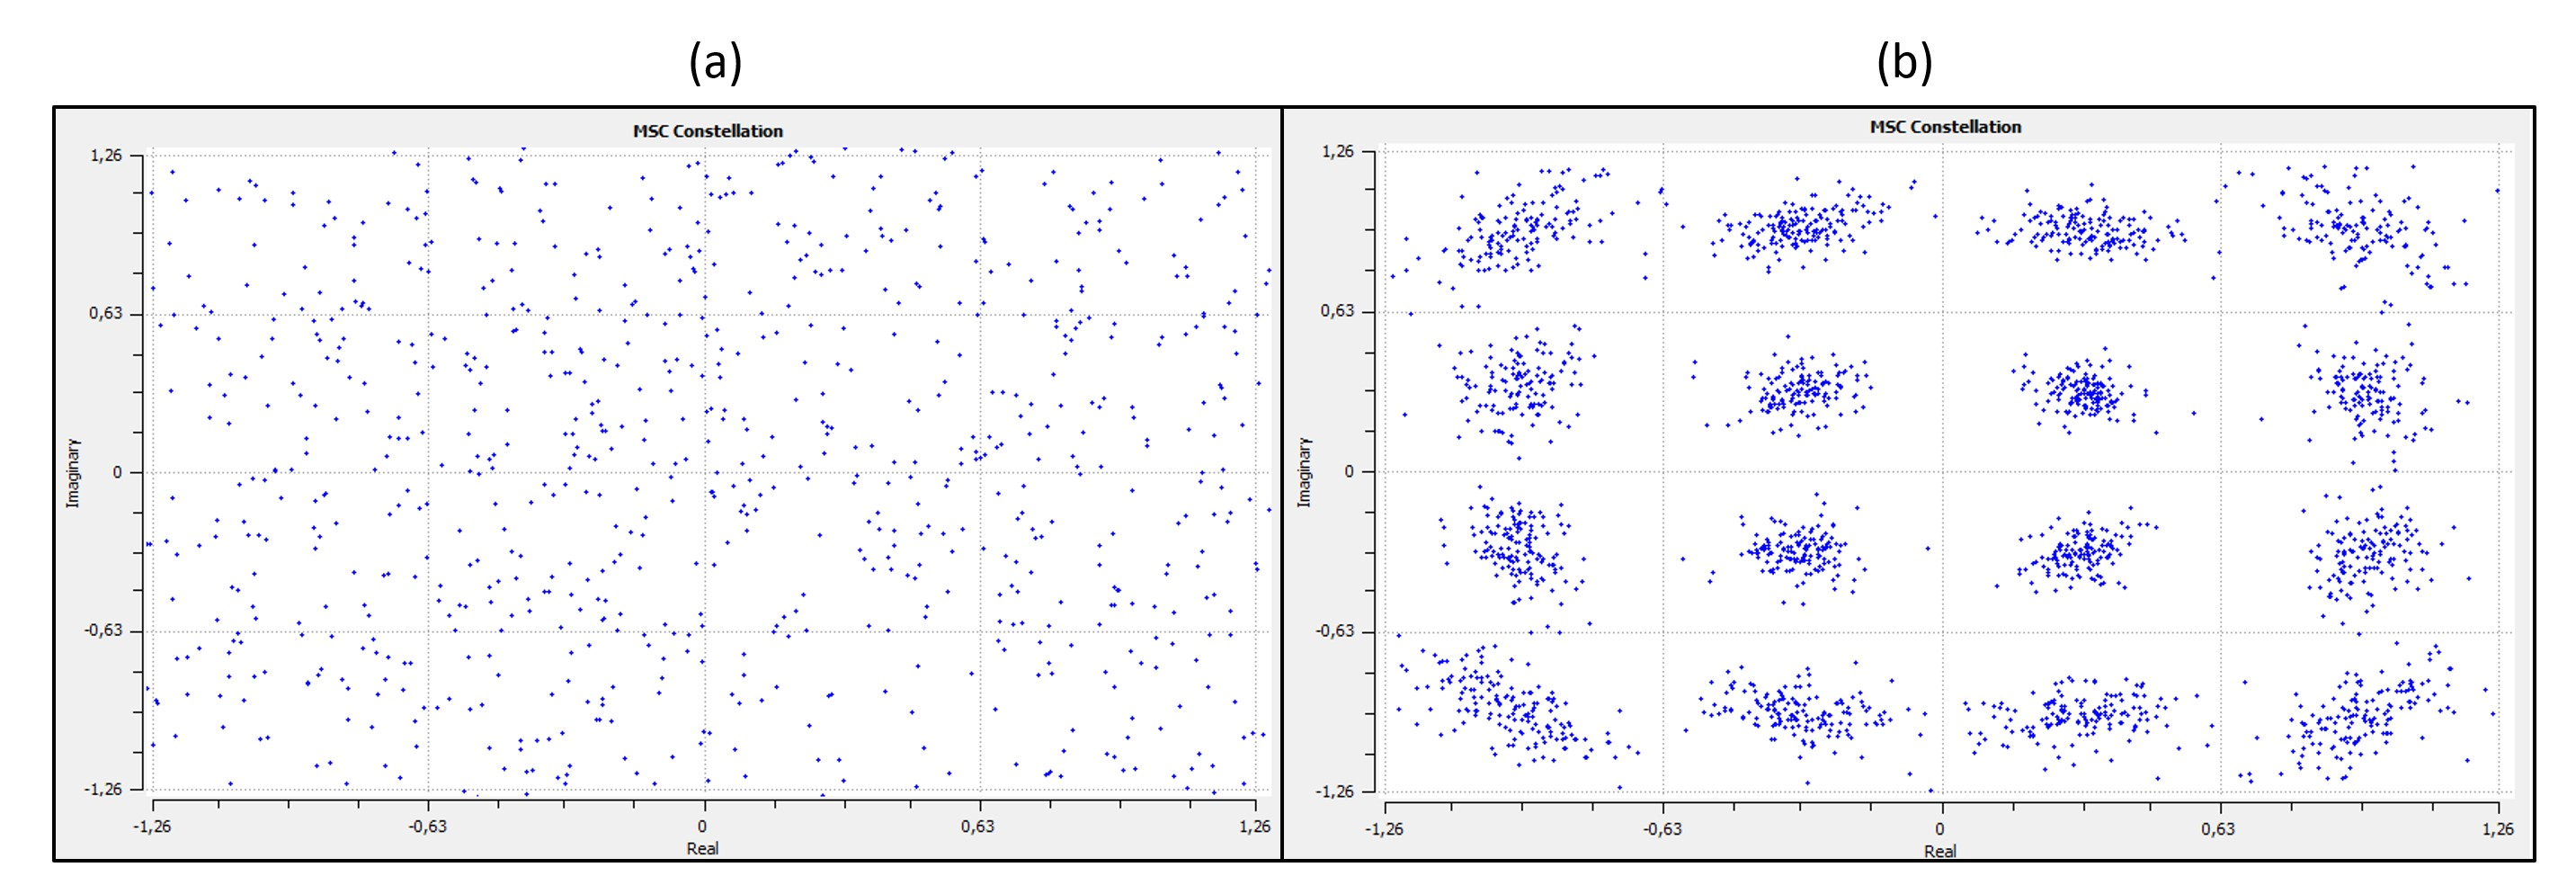
\includegraphics[width = 1 \textwidth]{msc.jpg}
	\caption[Konstellationsdiagramm des \gls{acr:MSC}]{Konstellationsdiagramm des \gls{acr:MSC}}\gls{online:Eigen}
	\label{fig:msc}
\end{figure}

\begin{figure}[H]
	\centering
	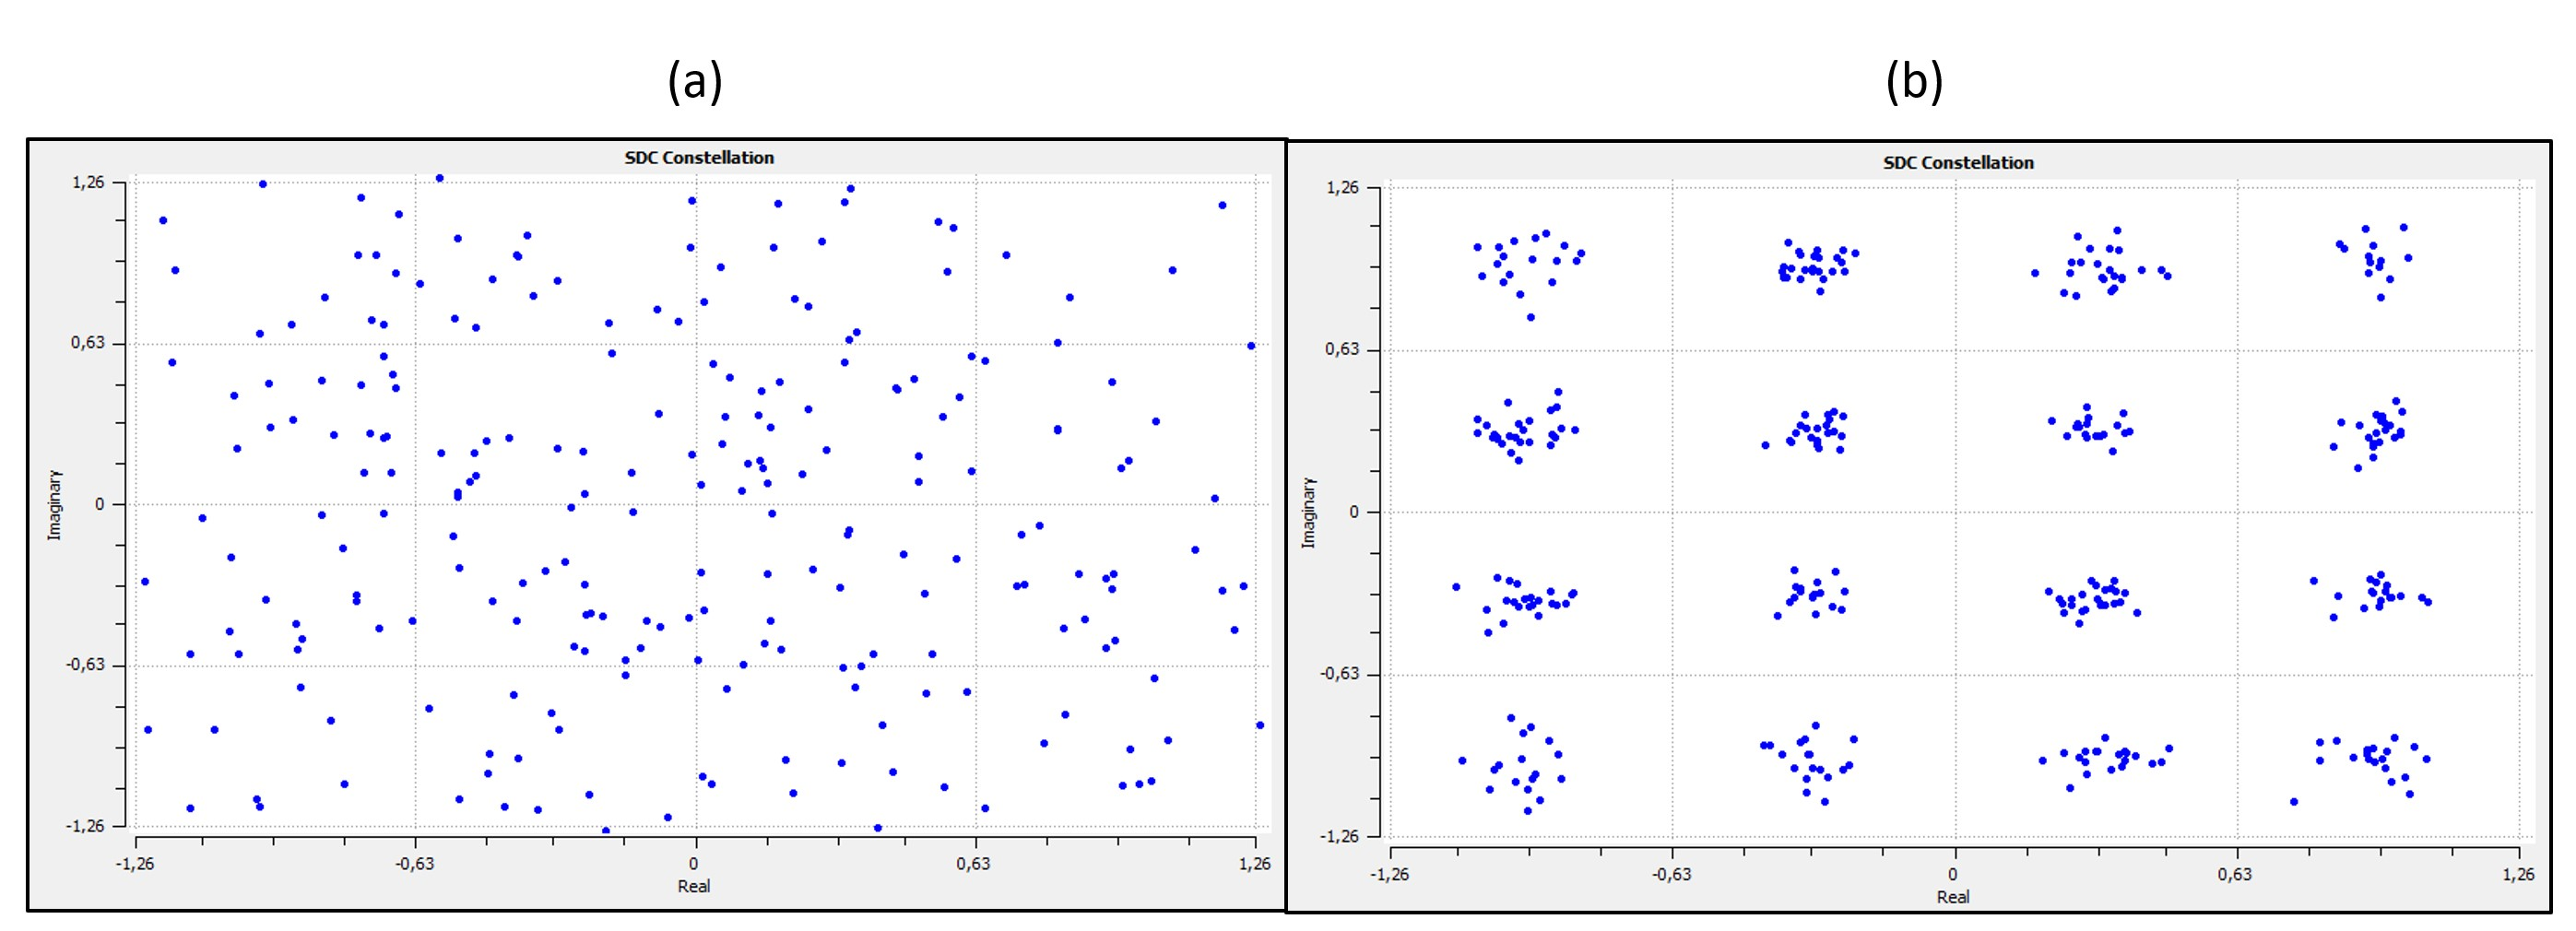
\includegraphics[width = 1 \textwidth]{sdc.jpg}
	\caption[Konstellationsdiagramm des \gls{acr:SDC}]{Konstellationsdiagramm des \gls{acr:FAC}}\gls{online:Eigen}
	\label{fig:sdc}
\end{figure}

\begin{figure}[H]
	\centering
	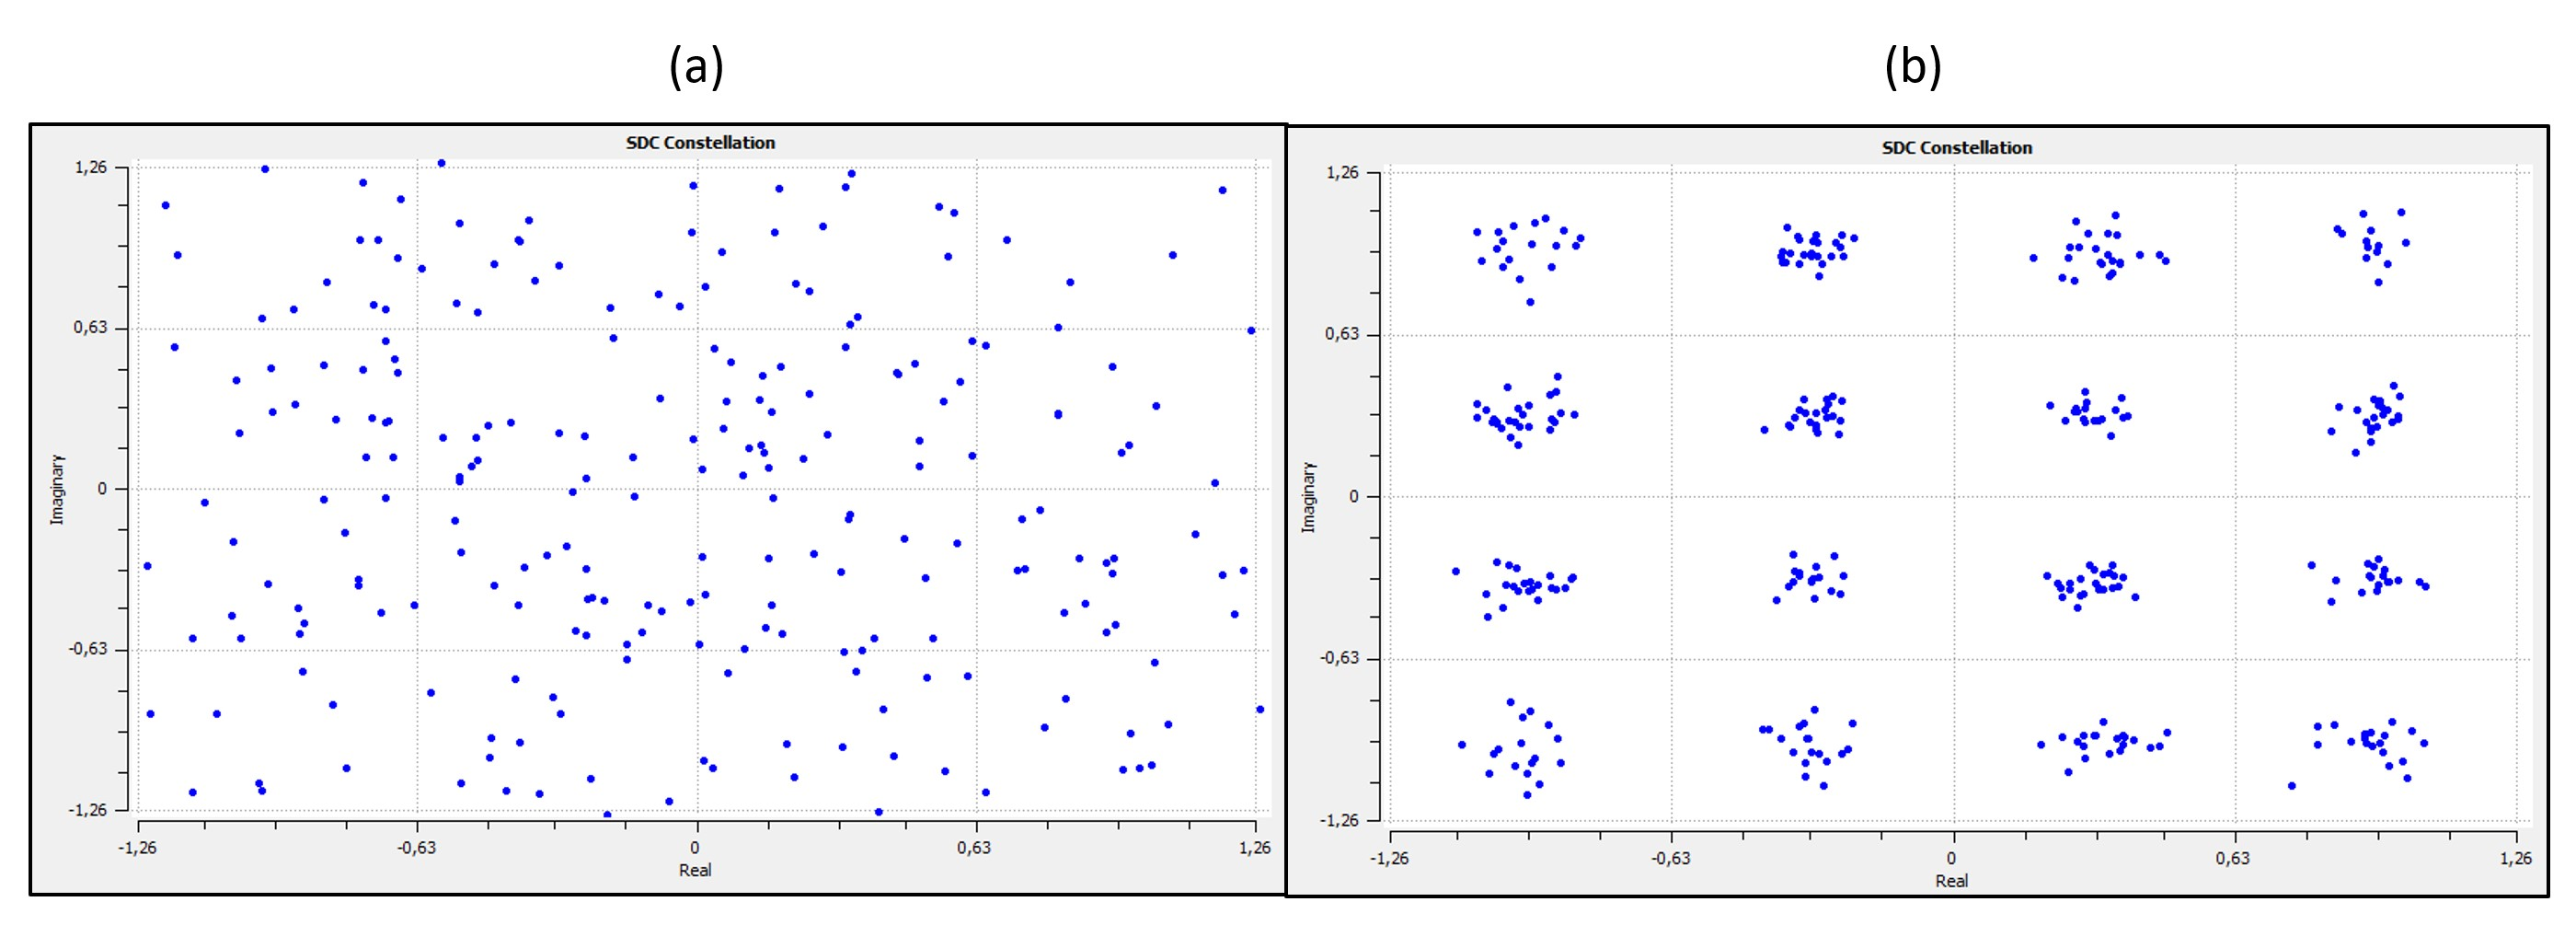
\includegraphics[width = 1 \textwidth]{fac.jpg}
	\caption[Konstellationsdiagramm des \gls{acr:FAC}]{Konstellationsdiagramm des \gls{acr:FAC}}\gls{online:Eigen}
	\label{fig:fac}
\end{figure}

Des weiteren wurde ein Test zur Detektierung der maximalen Übertragungsreichweite durchgeführt. Aufgrund der etwas begrenzten Datenrate, mussten bei der Übertragung Kompromisse zwischen einem höheren Fehlerschutz für eine bessere Empfangssicherheit und der damit zusammenhängenden niedrigeren Bitrate für die Audioübertragung gefunden werden. Die Einstellungen dieser Übertragung sind in Tabelle~\ref{tab:drmmax} dargestellt. Hierbei konnte eine maximale Reichweite von 11.24m erprobt werden.

\begin{table}[h]
	\begin{center}
		\begin{tabular}{cccc}
			\toprule
			\textbf{Datenrate [kbps]} & \textbf{Modulation}& \textbf{\gls{acr:MSC} Protection Level} & \textbf{\gls{acr:MSC} Interleaver Mode}\\
			\midrule
			
			14.56 &16-\gls{acr:QAM} & 1 & 2s long intervall\\
		
			\bottomrule
		\end{tabular}
		\caption{Einstellungen des Sendesignals bei maximaler Reichweite}\gls{online:dream}
		\label{tab:drmmax}
	\end{center}
\end{table}


 